% @author Lluis Gesa (lluis.gesa@uab.cat)
%
% Enginyeria Del Software
% -----------------------------------------------------------------------------------



% definim quin estil general volem per el document
\documentclass[11pt]{article}

% indiquem quins paquets amb funcionalitat extra volem fer servir
\usepackage{a4wide, amsmath, tabularx, colortbl, fancyhdr, graphicx, lastpage, caption}
\usepackage[utf8]{inputenc}

% Indiquem que comencem a definir el document i els seus continguts.
\begin{document}

% Definim valors i propietats, creem macros que ens ajudaran a
% agilitzar coses repetides:

\newcommand{\NomProjecte}{Perdidos en la ignorancia}
\newcommand{\NomDocument}{Especificaciones}
\newcommand{\IdentificadorDocument}{GG-SL-N-UC}
\newcommand{\VersioDocument}{v4.0}

% Fent servir propietas del paquet fancyhdr per crear una capçalera
% que es mostrarà cada pàgina
\pagestyle{fancy}
\fancyhead[LO,LE]{
\includegraphics[width = 3.5cm]{./imatges/uab-logo.png}}
\fancyhead[CO,CE]{\bf \NomProjecte \\ \vspace{\baselineskip}
  \NomDocument }
\fancyhead[RO,RE]{
{\bf Ref : \IdentificadorDocument} \\
Versió: \VersioDocument\\
Data: \today \\
Pag. \thepage ~of \pageref{LastPage}
}
\fancyfoot[LO,LE,CO,CE,RO,RE]{}
\textheight=19cm


%
% Creem la pàgina inicial :

% Insertem el nom del document en una taula centrada feng servir una
% font gran \huge

\begin{center}
\begin{tabular*}{15cm}{p{14.5cm}}
\\
\\
\\
\rowcolor[gray]{.9}\begin{center}\huge{\bf{\NomDocument}}\end{center}\\
\\
\end{tabular*}
\end{center}


%
% Insertem una taula que contindrà les abreviacions que hi hagi al
% nostre document
%
\small{%
\begin{center}
\begin{tabular}{|p{2cm}|p{4.75cm}|p{2cm}|p{4.75cm}|}
\hline
\multicolumn{4}{|>{\columncolor[gray]{.9}[2mm][2mm]}c|}{{\bf Abreviatures}} \\
\hline
UAB & Universitat Autonoma de Barcelona & ES & Enginyeria del Software \\
\hline
& & & \\
\hline
\end{tabular}
\end{center}
}

%
% Insertem una taula amb el historial de canvis del document
%
\small{%
\begin{center}
\begin{tabular}{|p{2cm}|p{2cm}|p{7.5cm}|p{2cm}|}
\hline
\multicolumn{4}{|>{\columncolor[gray]{.9}[2mm][2mm]}c|}{{\bf Historial de Revisions}} \\
\hline
{\bf Version} & {\bf Date} & {\bf Comments} & {\bf Autor} \\
\hline
1.0 & 08-Abril-2019 & Sprint 1 &
G43-2-02 \\
\hline
2.0 & 29-Abril-2019 & Sprint 2 &
G43-2-02 \\
\hline
3.0 & 12-Maig-2019 & Sprint 3 &
G43-2-02 \\
\hline
4.0 & 19-Maig-2019 & Sprint 4 &
G43-2-02 \\
\hline
\end{tabular}
\end{center}
}




% Insertem en una nova pàgina, els indexs : de continguts, de figures
% i de taules, les comandes \tableofcontents ,  \listoffigures,
% \listoftables són gestionades per els paquets fets servir, i per
% defecte escriuen els titols de la secció en angles, per canviar-los,
% hem de 'renovar les comandes' :

\renewcommand{\contentsname}{Índex de continguts}
\renewcommand{\listfigurename}{Índex de figures}
\renewcommand{\listtablename}{Índex de taules}

% Ara li diem al LaTeX que inserti la informació
\newpage
\tableofcontents
\listoffigures
\listoftables

% Insertem les seccions que volem
\newpage

\section{Introducció}\label{sec:intro}

\begin{flushleft}
En este documento se pretende detallar de forma minuciosa el comportamiento deseado de todos los casos de uso del sistema. De esta forma, será mucho más fácil saber que debe hacer cada módulo cuando se quiera dividir el conjunto de tareas a programar.\\


Además, esto ayuda a anticiparse a posibles necesidades y problemas, lo que agiliza el proyecto y ayuda a determinar con mayor exactitud las herramientas a utilizar y tiempo a invertir.\\


En este mismo documento se proporcionará los diagramas de casos de uso, para detectar de forma sencilla los actores que intervienen y sus respectivas acciones.\\
\end{flushleft}

\section{Use Case Diagram}\label{sec:uc}

Lorem ipsum dolor sit amet, consectetur adipiscing elit, sed do eiusmod tempor incididunt ut labore et dolore magna aliqua. Viverra orci sagittis eu volutpat odio. Quis hendrerit dolor magna eget. Elit scelerisque mauris pellentesque pulvinar pellentesque habitant. Viverra mauris in aliquam sem. Potenti nullam ac tortor vitae purus faucibus. Ut aliquam purus sit amet. Sed tempus urna et pharetra pharetra massa. Dolor sit amet consectetur adipiscing elit ut aliquam. Leo integer malesuada nunc vel risus commodo. Fau


  \begin{figure}[ht]
  \centering
  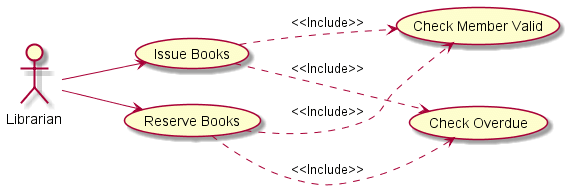
\includegraphics[width=1.1\textwidth]{./imatges/usecase.png}
  \label{fig:usecase}
   \end{figure}

\section{Caso de uso : 0001 - USUARIO: Identificación de usuario}\label{sec:uc0}
\subsection{Flujo de eventos}
\subsubsection{Básico}

\begin{enumerate}
\item Paso 1.
El usuario ingresa sus datos (usuario y contraseña).
\item Paso 2.
Si el login es correcto, se accede al sistema, si el usuario no existe, o bien, la contraseña es incorrecta se muestra un mensaje de error.
\end{enumerate}

\subsubsection{Alternativo}
Si se introduce tres veces seguidas una contraseña incorrecta, se bloqueará la cuenta durante 15 minutos.

\subsection{Precondiciones}
\begin{itemize}
\item No hay precondiciones.
\end{itemize}

\subsection{Postcondiciones}
\begin{itemize}
\item Se redirige al usuario al menú principal.
\end{itemize}



\section{Caso de uso : 0002 - ADMIN: Creación de mapas}\label{sec:uc0}
\subsection{Flujo de eventos}
\subsubsection{Básico}

\begin{enumerate}
\item Paso 1.
El administrador seleccionará la opción de crear mapa.
\item Paso 2.
El sistema le mostrará los diferentes niveles posibles (fácil, mediano, difícil).
\item Paso 3.
El administrador seleccionará la dificultad del mapa que creará.
\item Paso 4.
El sistema enviará al administrador al editor de mapas.
\item Paso 5.
El administrador creará el mapa des del editor de mapas y lo guardará.
\item Paso 6.
El sistema guardará el nuevo mapa.
\end{enumerate}

\subsection{Precondiciones}
\begin{itemize}
\item No hay precondiciones.
\end{itemize}

\subsection{Postcondiciones}
\begin{itemize}
\item Se redirige al usuario al menú principal.
\end{itemize}



\section{Caso de uso : 0003 - ADMIN: Modificación de mapas}\label{sec:uc0}
\subsection{Flujo de eventos}
\subsubsection{Básico}

\begin{enumerate}
\item Paso 1.
El administrador seleccionará la opción de modificar mapa.
\item Paso 2.
El sistema le mostrará los mapas disponibles.
\item Paso 3.
El administrador seleccionará el mapa a modificar.
\item Paso 4.
El sistema enviará al administrador al editor de mapas.
\item Paso 5.
El administrador modificará el mapa y lo guardará.
\item Paso 6.
El sistema guardará el nuevo mapa.
\end{enumerate}

\subsection{Precondiciones}
\begin{itemize}
\item No hay precondiciones.
\end{itemize}

\subsection{Postcondiciones}
\begin{itemize}
\item Se redirige al usuario al menú principal.
\end{itemize}


\section{Caso de uso : 0004 - ADMIN: Eliminación de mapas}\label{sec:uc0}
\subsection{Flujo de eventos}
\subsubsection{Básico}

\begin{enumerate}
\item Paso 1.
El administrador seleccionará la opción de eliminar mapa.
\item Paso 2.
El sistema le mostrará los mapas disponibles.
\item Paso 3.
El administrador seleccionará el mapa que desea eliminar.
\item Paso 4.
El sistema eliminará mapa.
\end{enumerate}

\subsection{Precondiciones}
\begin{itemize}
\item No hay precondiciones.
\end{itemize}

\subsection{Postcondiciones}
\begin{itemize}
\item Se redirige al usuario al menú principal.
\end{itemize}



\section{Caso de uso : 0005 - ADMIN: Eliminar cuentas}\label{sec:uc0}
\subsection{Flujo de eventos}
\subsubsection{Básico}

\begin{enumerate}
\item Paso 1.
El sistema mostrará las cuentas al administrador.
\item Paso 2.
El administrador seleccionará la cuenta a eliminar.
\item Paso 3.
El sistema borrará la cuenta.
\end{enumerate}

\subsection{Precondiciones}
\begin{itemize}
\item No hay precondiciones.
\end{itemize}

\subsection{Postcondiciones}
\begin{itemize}
\item Se redirige al usuario al menú principal.
\end{itemize}



\section{Caso de uso : 0006 - ADMIN: Crear cuentas}\label{sec:uc0}
\subsection{Flujo de eventos}
\subsubsection{Básico}

\begin{enumerate}
\item Paso 1.
El sistema pedirá los datos para la nueva cuenta (nombre del usuario, contraseña).
\item Paso 2.
El sistema comprobará que el usuario no exista. En el caso que ese nombre de usuario ya esté registrado, se mostrará un mensaje para que se escoja otro nombre no existente. También se comprobará que la contraseña cumpla los requisitos de seguridad, se mostrará un mensaje en caso que no cumpla las condiciones necesarias.
\item Paso 3.
El administrador especificará todas las características de la cuenta.
\item Paso 4.
El sistema creará la nueva cuenta.
\end{enumerate}

\subsubsection{Alternativo}
En caso de existir la cuenta, el sistema avisará con un error.

\subsection{Precondiciones}
\begin{itemize}
\item No hay precondiciones.
\end{itemize}

\subsection{Postcondiciones}
\begin{itemize}
\item Se redirige al usuario al menú principal.
\end{itemize}



\section{Caso de uso : 0007 - USUARIO: Empezar partida}\label{sec:uc0}
\subsection{Flujo de eventos}
\subsubsection{Básico}

\begin{enumerate}
\item Paso 1.
El usuario seleccionará la opción desde el menú principal.
\item Paso 2.
El sistema creará la nueva partida.
\end{enumerate}

\subsection{Precondiciones}
\begin{itemize}
\item No hay precondiciones.
\end{itemize}

\subsection{Postcondiciones}
\begin{itemize}
\item Se redirige al usuario al menú principal.
\end{itemize}



\section{Caso de uso : 0008 - USUARIO: Borrar su partida}\label{sec:uc0}
\subsection{Flujo de eventos}
\subsubsection{Básico}

\begin{enumerate}
\item Paso 1.
El usuario seleccionará la opción desde el menú principal.
\item Paso 2.
El sistema mostrará los mapas de ese usuario.
\item Paso 3.
El usuario seleccionará el mapa del cual desea borrar la partida.
\item Paso 4.
El sistema borrará el mapa.
\end{enumerate}

\subsection{Precondiciones}
\begin{itemize}
\item No hay precondiciones.
\end{itemize}

\subsection{Postcondiciones}
\begin{itemize}
\item Se redirige al usuario al menú principal.
\end{itemize}



\section{Caso de uso : 0009 - USUARIO: Continuar partida}\label{sec:uc0}
\subsection{Flujo de eventos}
\subsubsection{Básico}

\begin{enumerate}
\item Paso 1.
El usuario seleccionará la opción de continuar partida desde el menú principal.
\item Paso 2.
El sistema mostrará en que nivel se encuentra el usuario y su puntuación.
\item Paso 3.
El usuario decide si quiere seguir con la partida, o iniciar una de nueva.
\end{enumerate}

\subsection{Precondiciones}
\begin{itemize}
\item No hay precondiciones.
\end{itemize}

\subsection{Postcondiciones}
\begin{itemize}
\item Se redirige al usuario a la partida anterior o a una nueva.
\end{itemize}



\section{Caso de uso : 0010 - USUARIO: Gestión de partidas existentes}\label{sec:uc0}
\subsection{Flujo de eventos}
\subsubsection{Básico}

\begin{enumerate}
\item Paso 1.
El jugador tendrá en el menú la opción para gestionar sus partidas existentes.
\item Paso 2.
El sistema mostrará una lista de las partidas existentes.
\end{enumerate}

\subsection{Precondiciones}
\begin{itemize}
\item No hay precondiciones.
\end{itemize}

\subsection{Postcondiciones}
\begin{itemize}
\item Se le enseña al usuario las partidas existentes. 
\end{itemize}



\section{Caso de uso : 0011 - USUARIO: Nueva partida}\label{sec:uc0}
\subsection{Flujo de eventos}
\subsubsection{Básico}

\begin{enumerate}
\item Paso 1.
El usuario seleccionará la opción de partida nueva desde el menú principal. 
\item Paso 2.
El sistema permitirá al usuario iniciar una nueva partida sin que la anterior se borre (en el caso que la partida anterior haya sido guardada). 
\end{enumerate}

\subsection{Precondiciones}
\begin{itemize}
\item No hay precondiciones.
\end{itemize}

\subsection{Postcondiciones}
\begin{itemize}
\item Se inicia una partida nueva y la anterior queda registrada si el usuario lo desea. 
\end{itemize}



\section{Caso de uso : 0012 - ADMIN: Modificar contraseña}\label{sec:uc0}
\subsection{Flujo de eventos}
\subsubsection{Básico}

\begin{enumerate}
\item Paso 1.
El administrador seleccionará la opción de modificar contraseña desde el menú principal.
\item Paso 2.
El sistema mostrará todos los usuarios.
\item Paso 3.
El administrador seleccionará el usuario del cual quiere modificar la contraseña.
\item Paso 4.
El administrador modificará la contraseña del usuario.
\item Paso 5.
El sistema modificará la contraseña del usuario.
\end{enumerate}

\subsection{Precondiciones}
\begin{itemize}
\item No hay precondiciones.
\end{itemize}

\subsection{Postcondiciones}
\begin{itemize}
\item Se redirige al administrador al menú principal.
\end{itemize}



\section{Caso de uso : 0013 - ADMIN: Modificar ranking}\label{sec:uc0}
\subsection{Flujo de eventos}
\subsubsection{Básico}

\begin{enumerate}
\item Paso 1.
El administrador seleccionará la opción de modificar ranking desde el menú principal.
\item Paso 2.
El sistema mostrará el ranking.
\item Paso 3.
El administrador modificará el ranking.
\item Paso 4.
El sistema actualizará el ranking.
\end{enumerate}

\subsection{Precondiciones}
\begin{itemize}
\item No hay precondiciones.
\end{itemize}

\subsection{Postcondiciones}
\begin{itemize}
\item Se redirige al administrador al menú principal.
\end{itemize}



\section{Caso de uso : 0014 - USUARIO: Modificar datos}\label{sec:uc0}
\subsection{Flujo de eventos}
\subsubsection{Básico}

\begin{enumerate}
\item Paso 1.
El usuario seleccionará la opción de modificar datos de la cuenta desde el menú principal.
\item Paso 2.
El sistema mostrará los datos del usuario.
\item Paso 3.
El usuario modificará aquellos datos que crea necesarios.
\item Paso 4.
El sistema actualizará los nuevos datos.
\end{enumerate}

\subsection{Precondiciones}
\begin{itemize}
\item No hay precondiciones.
\end{itemize}

\subsection{Postcondiciones}
\begin{itemize}
\item Se redirige al usuario al menú principal.
\end{itemize}



\section{Caso de uso : 0015 - USUARIO: Eliminar datos}\label{sec:uc0}
\subsection{Flujo de eventos}
\subsubsection{Básico}

\begin{enumerate}
\item Paso 1.
El usuario seleccionará la opción de modificar datos de la cuenta.
\item Paso 2.
El sistema mostrará los datos del usuario.
\item Paso 3.
El usuario eliminará aquellos datos que crea necesarios.
\item Paso 4.
El sistema actualizará los datos eliminando aquellos seleccionados.
\end{enumerate}

\subsection{Precondiciones}
\begin{itemize}
\item No hay precondiciones.
\end{itemize}

\subsection{Postcondiciones}
\begin{itemize}
\item Se redirige al usuario al menú principal.
\end{itemize}



\section{Caso de uso : 0016 - SISTEMA: Gestionar niveles}\label{sec:uc0}
\subsection{Flujo de eventos}
\subsubsection{Básico}

\begin{enumerate}
\item Paso 1.
El sistema se engargará de gestionar los diferentes niveles del juego, de menor a mayor dificultad.
\end{enumerate}

\subsection{Precondiciones}
\begin{itemize}
\item No hay precondiciones.
\end{itemize}

\subsection{Postcondiciones}
\begin{itemize}
\item No hay postcondiciones.
\end{itemize}



\section{Caso de uso : 0017 - SISTEMA: Gestionar ranking}\label{sec:uc0}
\subsection{Flujo de eventos}
\subsubsection{Básico}

\begin{enumerate}
\item Paso 1.
El sistema se engaragrá de gestionar el ranking que irá de mayor a menor puntuación.
\end{enumerate}

\subsection{Precondiciones}
\begin{itemize}
\item No hay precondiciones.
\end{itemize}

\subsection{Postcondiciones}
\begin{itemize}
\item No hay postcondiciones.
\end{itemize}



\section{Caso de uso : 0018 - SISTEMA: Gestionar cuentas}\label{sec:uc0}
\subsection{Flujo de eventos}
\subsubsection{Básico}

\begin{enumerate}
\item Paso 1.
El sistema se engaragrá de gestionar todas las cuentas de usuario, guardando el nombre de usuario, su contraseña y los datos del usuario.
\end{enumerate}

\subsection{Precondiciones}
\begin{itemize}
\item No hay precondiciones.
\end{itemize}

\subsection{Postcondiciones}
\begin{itemize}
\item No hay postcondiciones.
\end{itemize}



\section{Caso de uso : 0019 - SISTEMA: Gestionar mapas}\label{sec:uc0}
\subsection{Flujo de eventos}
\subsubsection{Básico}

\begin{enumerate}
\item Paso 1.
El sistema se engargará de gestionar todos los mapas del juego según su dificultad.
\end{enumerate}

\subsection{Precondiciones}
\begin{itemize}
\item No hay precondiciones.
\end{itemize}

\subsection{Postcondiciones}
\begin{itemize}
\item No hay postcondiciones.
\end{itemize}



\section{Caso de uso : 0020 - ADMIN: Ver estado de los usuarios}\label{sec:uc0}
\subsection{Flujo de eventos}
\subsubsection{Básico}

\begin{enumerate}
\item Paso 1.
El administrador seleccionará la opción de estados de los usuarios desde el menú principal.
\item Paso 2.
El sistema mostrará en que estado se encuentra cada usuario (jugando, esperando o desconectado).
\end{enumerate}

\subsection{Precondiciones}
\begin{itemize}
\item No hay precondiciones.
\end{itemize}

\subsection{Postcondiciones}
\begin{itemize}
\item Se redirige al administrador al menú principal.
\end{itemize}



\section{Caso de uso : 0021 - USUARIO: Visualización del ranking}\label{sec:uc0}
\subsection{Flujo de eventos}
\subsubsection{Básico}

\begin{enumerate}
\item Paso 1.
El usuario seleccionará la opción de ver los ranking desde el menú principal. 
\item Paso 2.
El sistema mostrará dos opciones: ver ranking del jugador o ver el ranking de todos los usuarios del juego.
\item Paso 3.
El usuario seleccionará el ranking que desea ver.
\item Paso 4.
El sistema mostrará el ranking deseado por el usuario.
\item Paso 5.
El usuario decide si quiere seguir jugando o salir.
\end{enumerate}

\subsection{Precondiciones}
\begin{itemize}
\item No hay precondiciones.
\end{itemize}

\subsection{Postcondiciones}
\begin{itemize}
\item Se le muestra al usuario los rankings acumulados. 
\end{itemize}



\section{Caso de uso : 0022 - USUARIO: Modificación de los ajustes}\label{sec:uc0}
\subsection{Flujo de eventos}
\subsubsection{Básico}

\begin{enumerate}
\item Paso 1.
El usuario seleccionará la opción de modificar ajustes desde el menú principal. 
\item Paso 2.
El sistema permitirá al usuario hacer las modificaciones (de ajustes) que él crea convenientes. Activar o desactivar el volumen del juego i la vibración, escoger el idioma.
\item Paso 3.
El usuario podrá hacer las modificaciones necesarias y decidirá si quiere jugar una partida o salir.
\end{enumerate}

\subsection{Precondiciones}
\begin{itemize}
\item No hay precondiciones.
\end{itemize}

\subsection{Postcondiciones}
\begin{itemize}
\item El usuario hace modificaciones de ajustes mediante una opción en el menú.
\end{itemize}



\section{Caso de uso : 0023 - USUARIO: Volver al menú principal}\label{sec:uc0}
\subsection{Flujo de eventos}
\subsubsection{Básico}

\begin{enumerate}
\item Paso 1.
El usuario seleccionará la opción de menú principal. 
\item Paso 2.
El sistema redireccionará al usuario al menú principal. 
\item Paso 3.
El usuario podrá elegir alguna de las opciones existentes de este menú (el principal).
\end{enumerate}

\subsection{Precondiciones}
\begin{itemize}
\item No hay precondiciones.
\end{itemize}

\subsection{Postcondiciones}
\begin{itemize}
\item El usuario podrá acceder al menú principal.
\end{itemize}



\section{Caso de uso : 0024 - USUARIO: Salir del juego}\label{sec:uc0}
\subsection{Flujo de eventos}
\subsubsection{Básico}

\begin{enumerate}
\item Paso 1.
El usuario seleccionará la opción de salir del juego. 
\item Paso 2.
El juego se cerrará.
\end{enumerate}

\subsection{Precondiciones}
\begin{itemize}
\item No hay precondiciones.
\end{itemize}

\subsection{Postcondiciones}
\begin{itemize}
\item El usuario podrá salir del juego cuando quiera. 
\end{itemize}



\section{Caso de uso : 0025 - USUARIO: Guardado manual}\label{sec:uc0}
\subsection{Flujo de eventos}
\subsubsection{Básico}

\begin{enumerate}
\item Paso 1.
El usuario seleccionará la opción de guardar la partida actual.
\item Paso 2.
El usuario guardará la partida manualmente.  
\item Paso 3.
El sistema guardará la partida jugada hasta ese momento. 
\item Paso 4.
El usuario escogerá si salir del juego o continuar jugando. 
\end{enumerate}

\subsection{Precondiciones}
\begin{itemize}
\item No hay precondiciones.
\end{itemize}

\subsection{Postcondiciones}
\begin{itemize}
\item El usuario podrá guardar la partida manualmente. 
\end{itemize}



\section{Caso de uso : 0026 - ADMIN: Borrar juego}\label{sec:uc0}
\subsection{Flujo de eventos}
\subsubsection{Básico}

\begin{enumerate}
\item Paso 1.
El administrador podrá borrar el juego como administrador. 
\item Paso 2.
El sistema se borrará por completo. 
\end{enumerate}

\subsection{Precondiciones}
\begin{itemize}
\item No hay precondiciones.
\end{itemize}

\subsection{Postcondiciones}
\begin{itemize}
\item El administrador tendrá la opción de eliminar el juego.
\end{itemize}



\section{Caso de uso : 0027 - USUARIO: Comenzar partida de nuevo}\label{sec:uc0}
\subsection{Flujo de eventos}
\subsubsection{Básico}

\begin{enumerate}
\item Paso 1.
El usuario tendrá opción de empezar la partida de nuevo. 
\item Paso 2.
El sistema se actualizará con una nueva partida. 
\end{enumerate}

\subsection{Precondiciones}
\begin{itemize}
\item No hay precondiciones.
\end{itemize}

\subsection{Postcondiciones}
\begin{itemize}
\item El usuario empezará la misma partida de nuevo si desea. 
\end{itemize}



% \section{Traçabilitat}\label{sec:intro}

\begin{center}
\begin{tabular}{|c|c|c|}
\hline
{\cellcolor[gray]{.8} \bf Requeriment} & {\cellcolor[gray]{.8} \bf Cas d'ús} & {\cellcolor[gray]{.8} \bf Test}  \\
\hline
REQ-F-1-01 & CU-USUARI-01 & TP-U-01 \\
\hline
REQ-F-1-02 & CU-ADMIN-02 & TP-U-01 \\
\hline
REQ-F-1-03 & CU-ADMIN-03 & TP-U-01 \\
\hline
REQ-F-1-04 & CU-ADMIN-04 & TP-U-01 \\
\hline
REQ-F-1-05 & CU-USUARI-05 & TP-U-01 \\
\hline
REQ-F-1-06 & CU-USUARI-06 & TP-U-01 \\
\hline
REQ-F-1-07 & CU-ADMIN-07 & TP-U-01 \\
\hline
REQ-F-1-08 & CU-ADMIN-08 & TP-U-01 \\
\hline
REQ-F-1-09 & CU-USUARI-09 & TP-U-01 \\
\hline
REQ-F-1-10 & CU-SISTEMA-10 & TP-U-01 \\
\hline
REQ-F-1-11 & CU-SISTEMA-11 & TP-U-01 \\
\hline
REQ-F-1-12 & CU-ADMIN-12 & TP-U-01 \\
\hline
REQ-F-1-13 & CU-USUARI-13 & TP-U-01 \\
\hline
REQ-F-1-14 & CU-USUARI-14 & TP-U-01 \\
\hline
REQ-F-1-15 & CU-USUARI-15 & TP-U-01 \\
\hline

\end{tabular}
\captionof{table}{Matriu Traçabilitat}
\end{center}


% Finalitzem el document.
\end{document}
